\vfill

\tikzstyle{cluster}=[fill opacity=0.2,rounded corners,inner sep=0.1em]



\begin{figure}[h!]
  \centering
  \tikzstyle{nodestyle}=[inner sep=0.2em,outer sep=0em]
  \tikzstyle{every to}=[every node/.style={font=\scriptsize}]
  \begin{subfigure}[b]{.45\textwidth}
    \centering
    \begin{tikzpicture}
      \matrix (con) [matrix of math nodes,column sep=1.2em, row sep=1em, nodes={nodestyle}]
      {
		|(0)| 0 & |(1)| 1 & |(2)| 2 & |(3)| 3 & |(4)| 4 & |(5)| 5 & |(6)| 6 & |(7)| 7 & |(8)| 8 & |(9)| 9\\
      };
      \draw (0) to node [above] {2} (1) to node [above] {0.6} (2) to node [above] {1} (3) to node [above] {1} (4) to node [above] {1} (5) to node [above] {1} (6) to node [above] {1} (7) to node [above] {1} (8) to node [above] {1} (9);
      \node[cluster,fill=blue,fit=(0) (1)] {};
      \node[cluster,draw=red,fit=(0) (1) (2) (3) (4),inner sep=0.4em] {};
      %\node[cluster,draw=red,fit=(5) (6) (7) (8) (9),inner sep=0.4em] {};
    \end{tikzpicture}
    \caption{Minimum conductance: The sets $\{0,1,2,3,4\}$ and $\{5,6,7,8,9\}$ minimize the conductance to $\frac19$. In contrast,
our approach can return the desired cluster
$\{0,1\}$.}
    \label{fig:conductance}    
  \end{subfigure}
  \hfill
  \begin{subfigure}[b]{.45\textwidth}
    \centering
    \begin{tikzpicture}
      \matrix (DSP) [matrix of math nodes,column sep=1.2em, row sep=1em, nodes={nodestyle}]
      {
	|(0)| 0 & |(1)| 1 & |(2)| 2 & |(3)| 3 & |(4)| 4 \\
      };
      \draw (0) to node [above] {1} (1) (2) to node [above] {2} (3) to node [above] {1} (4);
      \node[cluster,fill=blue,fit=(0) (1)] {};
      \node[cluster,draw=red,fit=(2) (3)] {};
    \end{tikzpicture}
    \caption{Densest subgraphs: The set $\{0,1\}$ is a strong community returned by our method. However,
it is not a densest $2$-subgraph since $\{2,3\}$ has strictly more internal support. Hence, any
graph clustering algorithm that only returns densest subgraphs will fail to return the strong community.}
    \label{fig:DSP}    
  \end{subfigure}
  \\
  \begin{minipage}[b]{0.45\textwidth}
  \begin{subfigure}[b]{\textwidth}
    \centering
    \begin{tikzpicture}
      \matrix (con) [matrix of math nodes,column sep=1.2em, row sep=1em, nodes={nodestyle}]
      {
		|(0)| 0 & |(1)| 1 & |(2)| 2 & |(3)| 3 & |(4)| 4 & |(5)| 5 & |(6)| 6 & |(7)| 7 & |(8)| 8 & |(9)| 9\\
      };
      \draw (0) to node [above] {2} (1) to node [above] {0.6} (2) to node [above] {1} (3) to node [above] {1} (4) to node [above] {1} (5) to node [right] {1} (6) to node [above] {1} (7) to node [above] {1} (8) to node [above] {1} (9);
      \node[cluster,fill=blue,fit=(2) (3) (4) (5) (6) (7) (8) (9)] {};
      \node[cluster,draw=red,fit=(2) (3) (4) (5),inner sep=0.4em] {};
      \node[cluster,draw=red,fit=(6) (7) (8) (9),inner sep=0.4em] {};
      %\node[cluster,draw=red,fit=(5) (6) (7) (8) (9),inner sep=0.4em] {};
    \end{tikzpicture}
    \caption{Infomap: The sets $\{0,1\}$, $\{2,3,4,5\}$ and $\{6,7,8,9\}$ optimize the map equation~\cite{rosvall2008maps}. In contrast,
our approach can return the desired cluster $\{2,3,4,5,6,7,8,9\}$.}
    \label{fig:infomap}    
  \end{subfigure}\\
  \begin{subfigure}[b]{\textwidth}
    \centering
    \begin{tikzpicture}
      \matrix (con) [matrix of math nodes,column sep=1.2em, row sep=1em, nodes={nodestyle}]
      {
	|(0)| 0 & |(1)| 1 & |(2)| 2 & |(3)| 3 & |(4)| 4 & |(5)| 5\\
      };
      \draw (0) to node [above] {1} (1) to node [above] {2} (2) to node [above] {1} (3) to node [above] {0.5} (4) to node [above] {1} (5);
      % \node[cluster,fill=blue,fit=(0) (1)] {};
      \node[cluster,draw=red,fit=(0) (1) (2) (3),inner sep=0.4em] {};
      \node[cluster,draw=red,fit=(4) (5),inner sep=0.4em] {};
      %\node[cluster,draw=red,fit=(5) (6) (7) (8) (9),inner sep=0.4em] {};
    \end{tikzpicture}
    \caption{Infomap: will return \{\{0, 1, 2, 3\},\{4, 5\}\} but not the stronger community
	 $\{1,2\}$. In contrast, our formulation returns all the desired clusters parameterized by their strengths.}
    \label{fig:infomap2}
  \end{subfigure}
\end{minipage}
  \hfill
  \begin{subfigure}[b]{0.45\textwidth}
    % for drawing ring of clique
    % https://tex.stackexchange.com/questions/223854/drawing-a-ring-of-cliques-in-tikz-graphs/223902#223902
    \newcommand\single[2]{ % #1=labels, #2= n=number of nodes
      \foreach \x in {1,...,#2}{
        \pgfmathsetmacro{\ang}{360/#2}
        \pgfmathparse{(\x-1)*\ang}
        \node[draw,fill=red,circle,inner sep=1pt] (#1-\x) at (\pgfmathresult:4cm) {};
      }
      \foreach \x [count=\xi from 1] in {1,...,#2}{
        \foreach \y in {\x,...,#2}{
          \path (#1-\xi) edge[-] (#1-\y);
        }
      }
    }
    \centering
    \begin{tikzpicture}
    \begin{scope}[local bounding box=scope1]
    \node at (0,0){$n=5, m=30$};
    \end{scope}
    \foreach \s[count=\si from 0] in {0,45,90,...,360}{
    \begin{scope}[shift={($(scope1) +(\s:2)$)}, scale=0.1,rotate=\s+90]
    \single{\si}{5};
    \end{scope}
    }
    \foreach \i/\j in {1/2,2/3,3/4,4/5,5/6,6/7,7/8}
    \draw (\i-1)--(\j-3);
    %\draw[dotted,thick, outer sep=10pt] (8-1)--(1-3);
	 \def\dd{.13cm}
    \draw[dotted,thick, outer sep=10pt] ([xshift=-\dd, yshift=\dd]8-1.north)--([xshift=\dd, yshift=-\dd]1-3.south);
    \end{tikzpicture}
	 %
	 \hfill
    \begin{tikzpicture}
      \matrix (DSP) [matrix of math nodes,column sep=1.9em, row sep=2em, nodes={nodestyle}]
      {
		|(0)| 0 \\ |(1)| 1 \\ |(2)| 2 \\ |(3)| 3 \\
      };
		\draw (0) to node [left] {1} (1) (1) to node [left, rotate=0] {$0.6$} (2) to node [left] {1} (3);
      \node[cluster,inner sep=.3em,fill=blue,fit=(0) (1)] {};
      \node[cluster,inner sep=.3em,fill=blue,fit=(2) (3)] {};
      \node[cluster,inner sep=.9em, draw=red,fit=(0) (3)] {};
    \end{tikzpicture}
    \caption{Modularity: (Left) For a ring of cliques where $n$ is the clique size and $m$ is the number of
	 cliques, modularity method will group two consecutive cliques as one cluster due to the resolution limit.
	 On the other hand, our formulation can identify every clique. (Right) The
	 modularity score is minimized by the entire set, and so it fails to detect the more meaningful
	 communities $\Set{0,1}$ and $\Set{2,3}$, which can be identified using our formulation.}
    \label{fig:modularity_2}
  \end{subfigure}
  \hfill
  \vspace{-.5em}
  \caption{Examples of weighted graphs where our formulation can return more meaningful communities than existing methods. (Not all communities are highlighted.)}
  \label{fig:eg_for_graphs}
\end{figure}


\begin{figure}
    \centering
    \def\svgwidth{\columnwidth}
    \fontsize{10}{10}\selectfont
    \input{abcomm.pdf_tex}
    \hfill
    \vspace{-.5em}
    \caption{Strength-size plots showing existing algorithms fail to give strong communities of large sizes. We uses an LFR benchmark network~\cite{lancichinetti2009benchmarks} generated with $\mu=0.1$. Each black circle is a community obtain by our method, and the blue lines link to communities obtained by other methods that are smaller and has lower strength. All points below the red line (shaded in grey) are dominated by the trivial community consisting of all the nodes.}

  \label{fig:LFR}
\end{figure}


\begin{figure}[h!]
  \vspace{-1em}
  \centering
  \def\figsep{.2cm}
  \def\dist{1}
  \def\disty{.9}
  \begin{subfigure}[b]{.24\textwidth}
    \subcaptionbox{Our approach\label{fig:cnr-2000-ab}}{%
      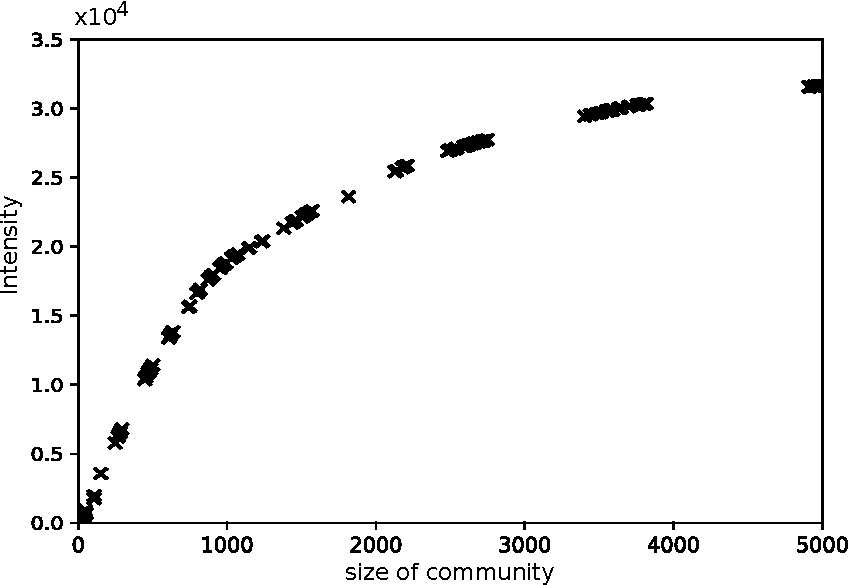
\includegraphics[width=\linewidth]{ab_cnr-2000.pdf}
    }
    % \label{fig:cnr-2000-ab}    
  \end{subfigure}
  \hfill
  \begin{subfigure}[b]{.24\textwidth}
    \subcaptionbox{SSM algorithm. (\cite{nagano2011size})\label{fig:cnr-2000-nagano}}{%
      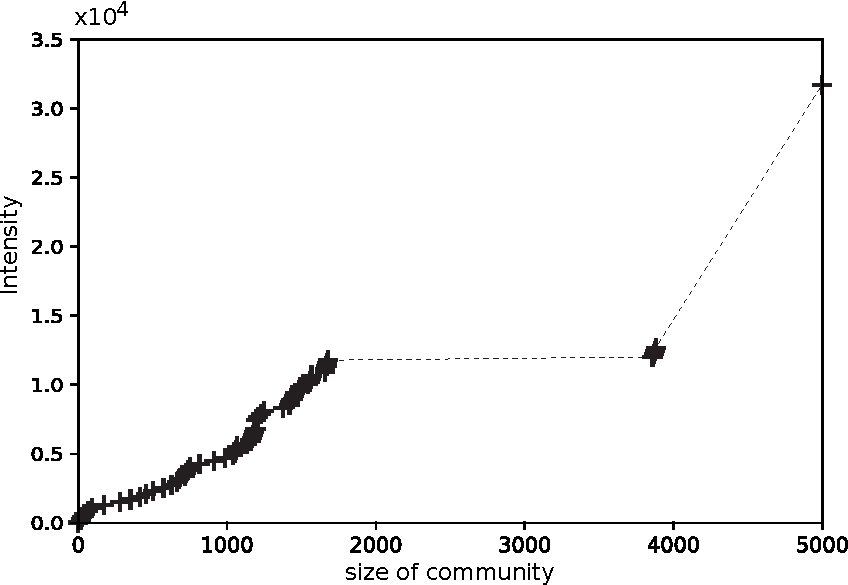
\includegraphics[width=\linewidth]{nagano_cnr-2000.pdf}
    }
    % \label{fig:cnr-2000-nagano}    
  \end{subfigure}
  \caption{Intensity vs. size plots showing that the proposed algorithm discovers more densest subgraphts of
	  large sizes. Our method retrieves 51 dense communities with cardinality $>$ 2000 while
	  the SSM algorithm in \cite{nagano2011size} only finds 2 such communities.}
  \label{fig:cnr-2000}
%  \caption{Intensity-size plots showing the proposed algorithm discovers more densest subgraphts of
%	  large sizes. Our method retrieves retrieve 51 dense communities with cardinality $>$ 2000 while
%	  the SSM algorithm in \cite{nagano2011size} only finds 2 such communities.}
  \label{fig:cnr-2000}
\end{figure}

